\documentclass[12pt]{report}
\usepackage[utf8]{inputenc}
\usepackage[russian]{babel}
%\usepackage[14pt]{extsizes}
\usepackage{listings}
\usepackage{graphicx}
\usepackage{amsmath,amsfonts,amssymb,amsthm,mathtools} 

% Для листинга кода:
\lstset{ %
language=C++,                 % выбор языка для подсветки (здесь это С)
basicstyle=\small\sffamily, % размер и начертание шрифта для подсветки кода
numbers=left,               % где поставить нумерацию строк (слева\справа)
numberstyle=\tiny,           % размер шрифта для номеров строк
stepnumber=1,                   % размер шага между двумя номерами строк
numbersep=5pt,                % как далеко отстоят номера строк от подсвечиваемого кода
showspaces=false,            % показывать или нет пробелы специальными отступами
showstringspaces=false,      % показывать или нет пробелы в строках
showtabs=false,             % показывать или нет табуляцию в строках
frame=single,              % рисовать рамку вокруг кода
tabsize=2,                 % размер табуляции по умолчанию равен 2 пробелам
captionpos=t,              % позиция заголовка вверху [t] или внизу [b] 
breaklines=true,           % автоматически переносить строки (да\нет)
breakatwhitespace=false, % переносить строки только если есть пробел
escapeinside={\#*}{*)}   % если нужно добавить комментарии в коде
}

% Для измененных титулов глав:
\usepackage{titlesec, blindtext, color} % подключаем нужные пакеты
\definecolor{gray75}{gray}{0.75} % определяем цвет
\newcommand{\hsp}{\hspace{20pt}} % длина линии в 20pt
% titleformat определяет стиль
\titleformat{\chapter}[hang]{\Huge\bfseries}{\thechapter\hsp\textcolor{gray75}{|}\hsp}{0pt}{\Huge\bfseries}


% plot
\usepackage{pgfplots}
\usepackage{filecontents}
\usetikzlibrary{datavisualization}
\usetikzlibrary{datavisualization.formats.functions}
\begin{filecontents}{LevR.dat}
100 45504
200 344852
300 1626090
400 4410053
500 8809530
600 15523926
700 27314819
800 36896674
900 151438792
1000 253111941
\end{filecontents}

\begin{filecontents}{LevT.dat}
100 50613
200 254889
300 1164803
400 3277843
500 6466829
600 10441740
700 20235150
800 27982176
900 115139281
1000 199701561
\end{filecontents}

\begin{filecontents}{DamLevR.dat}
100 22663
200 189215
300 937882
400 2605948
500 5077237
600 9041331
700 15047492
800 20829956
900 85256627
1000 158414218
\end{filecontents}



\begin{filecontents}{LevR1.dat}
101 45393
201 386372
301 1557256
401 4538718
501 9009942
601 15214595
701 26603522
801 37648086
901 139235577
1001 278285719
\end{filecontents}

\begin{filecontents}{LevT1.dat}
101 35265
201 364594
301 1113414
401 3314034
501 6511456
601 11947585
701 20274021
801 26844301
901 136919210
1001 212082553
\end{filecontents}

\begin{filecontents}{DamLevR1.dat}
101 38152
201 196174
301 919775
401 2652528
501 5171817
601 10328122
701 15001586
801 20867237
901 108043316
1001 165932409
\end{filecontents}



\begin{document}
%\def\chaptername{} % убирает "Глава"
\begin{titlepage}
	\centering
	{\scshape\LARGE МГТУ им. Баумана \par}
	\vspace{3cm}
	{\scshape\Large Лабораторная работа №2\par}
	\vspace{0.5cm}	
	{\scshape\Large По курсу: "Анализ алгоритмов"\par}
	\vspace{1.5cm}
	{\huge\bfseries Алгоритмы умножения матриц\par}
	\vspace{2cm}
	\Large Работу выполнила: Лаврова Анастасия, ИУ7-55Б\par
	\vspace{0.5cm}
	\LargeПреподаватели:  Волкова Л.Л., Строганов Ю.В.\par

	\vfill
	\large \textit {Москва, 2019} \par
\end{titlepage}

\tableofcontents

\newpage
\chapter*{Введение}
\addcontentsline{toc}{chapter}{Введение}
Цель работы: изучение алгоритмов умножения матриц. В данной лабораторной работе рассматривается стандартный алгоритм умножения матриц, алгоритм Винограда и модифицированный алгоритм Винограда.  Также требуется изучить рассчет сложности алгоритмов, получить навыки в улучшении алгоритмов.
Эти алгоритмы активно применяются во всех областях, применяющих линейную алгебру, таких как:
\begin{itemize}
	\item компьютерная графика
	\item физика
	\item экономика
\end{itemize}
и так далее.\\

В ходе лабораторной работы предстоит:
\begin{itemize}
	\item Изучить алгоритмы умножения матриц: стандартный и алгоритм Винограда 
	\item Улучшить алгоритм Винограда 
	\item Дать теоретическую оценку базового алгоритма умножения матриц, алгоритма Винограда и улучшенного алгоритма Винограда 
	\item Реализовать три алгоритма умножения матриц на одном из языков программирования  
	\item Сравнить алгоритмы умножения матриц  
\end{itemize}





\chapter{Аналитическая часть}
Матрица - математический объект, эквивалентный двумерному массиву. Числа располагаются в матрице по строкам и столбцам. Если число столбцов в первой матрице совпадает с числом строк во второй, то эти две матрицы можно перемножить. У произведения будет столько же строк, сколько в первой матрице, и столько же столбцов, сколько во второй.
	    
\section{Классический алгоритм умножения матриц}
Пусть даны две прямоугольные матрицы А и В размерности m на n и n на l соответсвенно: 
\[ \begin{bmatrix}
a_{1,1} & ... & a_{1,n} \\
... & ... & ... \\
a_{m,1} & ... & a_{m,n} \\
\end{bmatrix} \]\\

\[ \begin{bmatrix}
b_{1,1} & ... & b_{1,l} \\
... & ... & ... \\
b_{n,1} & ... & b_{n,l} \\
\end{bmatrix} \]\\

В результате получим матрицу C размерности m на l:
	
\[ \begin{bmatrix}
c_{1,1} & ... & c_{1,l} \\
... & ... & ... \\
c_{m,1} & ... & c_{m,l} \\
\end{bmatrix} \]\\


$c_{i,j} = \sum\limits_{r=1}^n a_{i,r}\cdot b_{r,j}$ называется произведением матриц A и B.


\section{Алгоритм Винограда}
Рассмотрим два вектора $V = (v1, v2, v3, v4)$ и $W = (w1, w2, w3, w4)$. Их скалярное произведение равно: 

$ V \cdot W=v_1 \cdot w_1 + v_2 \cdot w_2 + v_3 \cdot w_3 + v_4 \cdot w_4$ \\

Это равенство можно переписать в виде: \\
$V \cdot W=(v_1 + w_2) \cdot (v_2 + w_1) + (v_3 + w_4) \cdot (v_4 + w_3) - v_1 \cdot v_2 - v_3 \cdot v_4 - w_1 \cdot w_2 - w_3 \cdot w_4$\\

Менее очевидно, что выражение в правой части последнего равенства допускает предварительную обработку: его части можно вычислить заранее и запомнить для каждой строки первой матрицы и для каждого столбца второй. 
Это означает, что над предварительно обработанными элементами нам придется выполнять лишь первые два умножения и последующие пять сложений, а также дополнительно два сложения. 

\subsection{Вывод}
Были рассмотрены поверхностно алгоритмы классического умножения матриц и алгоритм Винограда, основная разница которого — наличие предварительной обработки, а также уменьшение количества операций умножения.


\chapter{Конструкторская часть}
\textbf{Требования к вводу:}\\
На вход подаются две матрицы и их размерности\\
\textbf{Требования к программе:}\\
Корректное умножение двух матриц \\

\begin{figure}[h]
\centering
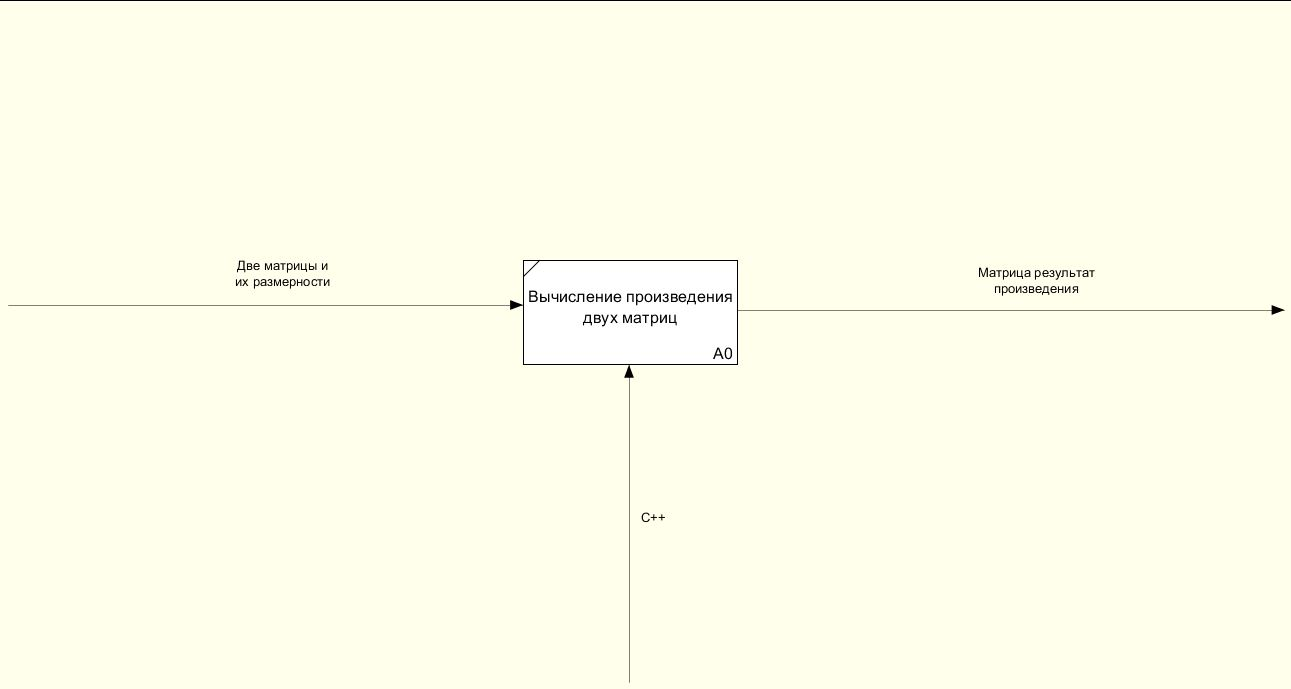
\includegraphics[width=1\linewidth]{idef.jpg}
\caption{IDEF0-диаграмма, описывающая алгоритм нахождения произведения двух матриц}
\label{fig:mpr}
\end{figure}

\section{Схемы алгоритмов}
В данной части будут рассмотрены схемы алгоритмов.

\begin{figure}[!htbp]
\centering
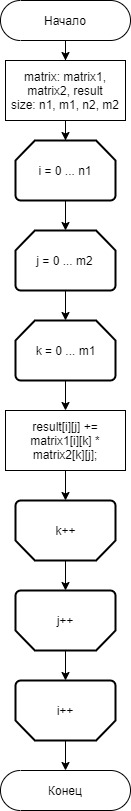
\includegraphics[scale=0.7]{alg1.jpg}
\caption{Схема классического алгоритма умножения матриц}
\label{fig:mpr}
\end{figure}

\begin{figure}[!htbp]
\centering
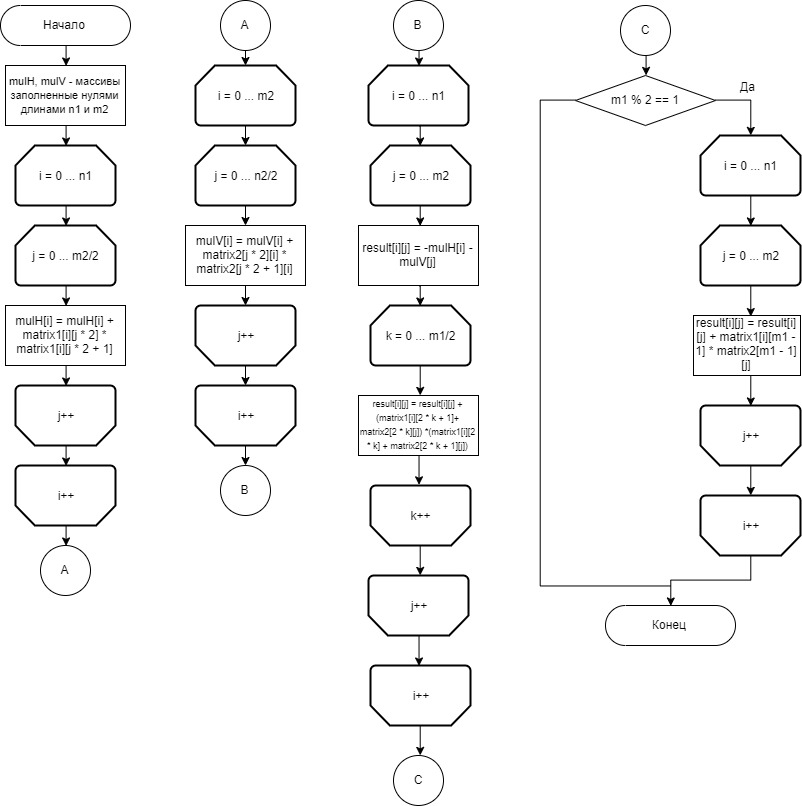
\includegraphics[scale=0.6]{alg2.jpg}
\caption{Схема алгоритма Винограда}
\label{fig:mpr}
\end{figure}


\begin{figure}[!htbp]
\centering
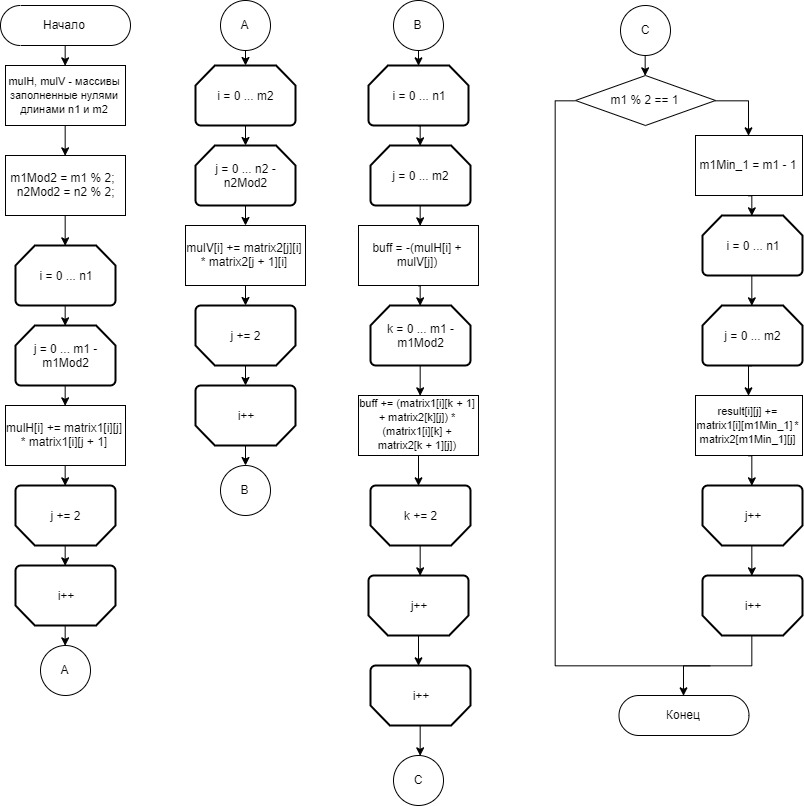
\includegraphics[scale=0.6]{alg3.jpg}
\caption{Схема оптимизированного алгоритма Винограда}
\label{fig:mpr}
\end{figure}

\section{Трудоемкость алгоритмов}
Введем модель трудоемкости для оценки алгоритмов: 
\begin{itemize}
	\item базовые операции стоимостью 1 — +, -, *, /, =, ==, <=, >=, !=, +=, []
	\item оценка трудоемкости цикла for от 0 до N с шагом 1 $F_{for} = 2 + N \cdot (2 + F_{body})$, где $F_{body}$ - тело цикла
	\item стоимость условного перехода применим за 0, стоимость вычисления условия остаётся
\end{itemize}

Оценим трудоемкость алгоритмов по коду программы

\subsection{Классический алгоритм}
Рассмотрим трудоемкость классического алгоритма:\\

$10MNQ + 4MQ + 4 M + 2$ \\


\subsection{Алгоритм Винограда}

Рассмотрим трудоемкость алгоритма Винограда:\\

Трудоемкость алгоритма Винограда:\\

Первый цикл: $15/2 \cdot M  N + 5 \cdot M + 2$ \\

Второй цикл: $15/2 \cdot M  N + 5 \cdot M + 2$\\

Третий цикл: $13 \cdot M  N Q + 12 \cdot M Q + 4 \cdot M + 2$\\

Условный переход: $\begin{bmatrix}
             2    &&, \text{в случае невыполнения условия}\\
             15 \cdot QM + 4 \cdot M + 2 &&, \text{в случае выполнения условия}\\
           \end{bmatrix} $ \\

Итого: $15/2 \cdot M  N + 5 \cdot M + 2 + 15/2 \cdot M  N + 5 \cdot M + 2 + 13 \cdot M  N Q + 12 \cdot M Q + 4 \cdot M + 2 +
       \begin{bmatrix}
             2    &&, \text{в случае невыполнения условия}\\
             15 \cdot QM + 4 \cdot M + 2 &&, \text{в случае выполнения условия}\\
           \end{bmatrix} $ \\

\subsection{Оптимизированный алгоритм Винограда}

Рассмотрим трудоемкость алгоритма Винограда:\\

Трудоемкость алгоритма Винограда:\\

Первый цикл: $11/2 \cdot M  N + 4 \cdot M + 2$ \\

Второй цикл: $11/2 \cdot M  N + 4 \cdot M + 2$\\

Третий цикл: $17/2 \cdot M  N Q + 9 \cdot M Q + 4 \cdot M + 2$\\

Условный переход: $\begin{bmatrix}
             1    &&, \text{в случае невыполнения условия}\\
             10 \cdot QM + 4 \cdot M + 2 &&, \text{в случае выполнения условия}\\
           \end{bmatrix} $ \\

Итого: $11/2 \cdot M  N + 4 \cdot M + 2 + 11/2 \cdot M  N + 4 \cdot M + 2 + 15/2 \cdot M  N Q + 9 \cdot M Q + 4 \cdot M + 2 +
       \begin{bmatrix}
             1    &&, \text{в случае невыполнения условия}\\
             10 \cdot QM + 4 \cdot M + 2 &&, \text{в случае выполнения условия}\\
           \end{bmatrix} $ \\



\chapter{Технологическая часть}
\section{Выбор ЯП}
Для реализации программ я выбрала язык программирования C++, так имею большой опыт работы с ним. Среда разработки - Visual Studio. \\

Для замера процессорного времени используется функция, возвращающая количество тиков.\\

\begin{lstlisting}[label=some-code,caption=Функция получения тиков]
unsigned long long getTicks(void)
{
    unsigned long long d;
    __asm__ __volatile__ ("rdtsc" : "=A" (d) );
    return d;
}

\end{lstlisting}

\section{Реализация алгоритма}

\begin{lstlisting}[label=some-code,caption=Функция классического умножения матриц]
int** mult_m(int** matrix1, int n1, int m1, int** matrix2, int n2, int m2)
{
	int** result = NULL;
	if (matrix1 && matrix2 && m1 == n2)
	{
		result = new_m(n1, m2);
		for (int i = 0; i < n1; i++)
			for (int j = 0; j < m2; j++)
				for (int k = 0; k < m1; k++)
					result[i][j] += matrix1[i][k] * matrix2[k][j];
	}
	return result;
}
\end{lstlisting}


\begin{lstlisting}[label=some-code,caption=Алгоритм Винограда]
int** Vinograd(int** matrix1, int n1, int m1, int** matrix2, int n2, int m2)
{
	int* mulH = (int*)malloc(n1 * sizeof(int));
	for (int i = 0; i < n1; i++)
		mulH[i] = 0;

	int* mulV = (int*)malloc(m2 * sizeof(int));
	for (int i = 0; i < m2; i++)
		mulV[i] = 0;

	int** result = new_m(n1, m2);

	for (int i = 0; i < n1; i++)
	{
		for (int j = 0; j < m1 / 2; j++)
		{
			mulH[i] = mulH[i] + matrix1[i][j * 2] * matrix1[i][j * 2 + 1];
		}
	}

	for (int i = 0; i < m2; i++)
	{
		for (int j = 0; j < n2 / 2; j++)
		{
			mulV[i] = mulV[i] + matrix2[j * 2][i] * matrix2[j * 2 + 1][i];
		}
	}

	for (int i = 0; i < n1; i++)
	{
		for (int j = 0; j < m2; j++)
		{
			result[i][j] = -mulH[i] - mulV[j];
			for (int k = 0; k < m1 / 2; k++)
			{
				result[i][j] = result[i][j] + (matrix1[i][2 * k + 1]+ matrix2[2 * k][j]) * (matrix1[i][2 * k] + matrix2[2 * k + 1][j]);
			}
		}
	}

	if (m1 % 2)
	{
		for (int i = 0; i < n1; i++)
		{
			for (int j = 0; j < m2; j++)
			{
				result[i][j] = result[i][j] + matrix1[i][m1 - 1] * matrix2[m1 - 1][j];
			}
		}
	}
	free(mulH);
	free(mulV);
	return result;
}
\end{lstlisting}


\begin{lstlisting}[label=some-code,caption=Оптимизированный алгоритм Винограда]
int** Vinograd_optim(int** matrix1, int n1, int m1, int** matrix2, int n2, int m2)
{
	int* mulH = (int*)malloc(n1 * sizeof(int));
	for (int i = 0; i < n1; i++)
		mulH[i] = 0;

	int* mulV = (int*)malloc(m2 * sizeof(int));
	for (int i = 0; i < m2; i++)
		mulV[i] = 0;

	int** result = new_m(n1, m2);

	int m1Mod2 = m1 % 2;
	int n2Mod2 = n2 % 2;

	for (int i = 0; i < n1; i++)
	{
		for (int j = 0; j < (m1 - m1Mod2); j += 2)
		{
			mulH[i] += matrix1[i][j] * matrix1[i][j + 1];
		}
	}

	for (int i = 0; i < m2; i++)
	{
		for (int j = 0; j < (n2 - n2Mod2); j += 2)
		{
			mulV[i] += matrix2[j][i] * matrix2[j + 1][i];
		}
	}

	for (int i = 0; i < n1; i++)
	{
		for (int j = 0; j < m2; j++)
		{
			int buff = -(mulH[i] + mulV[j]);
			for (int k = 0; k < (m1 - m1Mod2); k += 2)
			{
				buff += (matrix1[i][k + 1] + matrix2[k][j]) * (matrix1[i][k] + matrix2[k + 1][j]);
			}
			result[i][j] = buff;
		}
	}

	if (m1Mod2)
	{
		int m1Min_1 = m1 - 1;
		for (int i = 0; i < n1; i++)
		{
			for (int j = 0; j < m2; j++)
			{
				result[i][j] += matrix1[i][m1Min_1]	* matrix2[m1Min_1][j];
			}
		}
	}

	free(mulH);
	free(mulV);
	return result;
}
\end{lstlisting}

\subsection{Оптимизация алгоритма Винограда}
\begin{enumerate}
	\item Избавиться от деления в цикле;
	\item Замена $mulH[i] = mulH[i] + …$ на $mulH[i] += …$ (аналогично для $mulV[i]$);
	\begin{lstlisting}[label=some-code,caption=Оптимизации алгоритма Винограда №1 и №2]
int m1Mod2 = m1 % 2;
int n2Mod2 = n2 % 2;

	for (int i = 0; i < n1; i++)
	{
		for (int j = 0; j < (m1 - m1Mod2); j += 2)
		{
			mulH[i] += matrix1[i][j] * matrix1[i][j + 1];
		}
	}

	for (int i = 0; i < m2; i++)
	{
		for (int j = 0; j < (n2 - n2Mod2); j += 2)
		{
			mulV[i] += matrix2[j][i] * matrix2[j + 1][i];
		}
	}
\end{lstlisting}

	\item Накопление результата в буфер, а вне цикла сброс буфера в ячейку матрицы
	\begin{lstlisting}[label=some-code,caption=Оптимизации алгоритма Винограда №3]
for (int i = 0; i < n1; i++)
	{
		for (int j = 0; j < m2; j++)
		{
			int buff = -(mulH[i] + mulV[j]);
			for (int k = 0; k < (m1 - m1Mod2); k += 2)
			{
				buff += (matrix1[i][k + 1] + matrix2[k][j]) * (matrix1[i][k] + matrix2[k + 1][j]);
			}
			result[i][j] = buff;
		}
	}
\end{lstlisting}

\end{enumerate}




\chapter{Исследовательская часть}

\section{Сравнительный анализ на основе замеров времени работы алгоритмов}

Был проведен замер времени работы каждого из алгоритмов.\\
Первый эксперимент производится для лучшего случая на матрицах с размерами от 100 x 100 до 1000 x 1000 c шагом 100. \\


\begin{tikzpicture}

\begin{axis}[
    	axis lines = left,
    	xlabel={Размер матрицы},
    	ylabel={Время (тики)},
    	xmin=100, xmax=1000,
    	ymin=0, ymax=300000000,
	legend pos=north west,
	ymajorgrids=true
]
\addplot[color=red, mark=square] table[x index=0, y index=1] {LevR.dat}; 
\addplot[color=green, mark=square] table[x index=0, y index=1] {DamLevR.dat};
\addplot[color=blue, mark=square] table[x index=0, y index=1] {LevT.dat};

\addlegendentry{Стандартный}
\addlegendentry{Оптимизированный алг.}
\addlegendentry{Алг. Винограда}
\end{axis}
\end{tikzpicture}

\begin{center}
  	Рисунок 4.1. График времени работы алгоритмов на матрицах четной размерности
	\end{center}
	
Второй эксперимент производится для худшего случая, когда поданы матрицы с нечетными размерами от 101 x 101 до 1001 x 1001 c шагом 100. \\


\begin{tikzpicture}

\begin{axis}[
    	axis lines = left,
    	xlabel={Размер матрицы},
    	ylabel={Время (тики)},
    	xmin=100, xmax=1000,
    	ymin=0, ymax=300000000,
	legend pos=north west,
	ymajorgrids=true
]
\addplot[color=red, mark=square] table[x index=0, y index=1] {LevR1.dat}; 
\addplot[color=green, mark=square] table[x index=0, y index=1] {DamLevR1.dat};
\addplot[color=blue, mark=square] table[x index=0, y index=1] {LevT1.dat};

\addlegendentry{Стандартный}
\addlegendentry{Оптимизированный алг.}
\addlegendentry{Алг. Винограда}
\end{axis}
\end{tikzpicture}

\begin{center}
  	Рисунок 4.2. График времени работы алгоритмов на матрицах нечетной размерности
	\end{center}


\par
По результатам тестирования все рассматриваемые алгоритмы реализованы правильно. Самым медленным алгоритмом оказался алгоритм классического умножения матриц, а самым быстрым — оптимизированный алгоритм Винограда

\section{Тестовые данные}

Проверка работы алгоритмов на примерах:
\begin{itemize}
	\item матрицы размерностью 0 на 0
	\item матрицы размерностью 1 на 1
	\item матрицы размерностью 2 на 2
	\item матрицы размерностью 3 на 3
\end{itemize}

\begin{figure}[h]
\centering
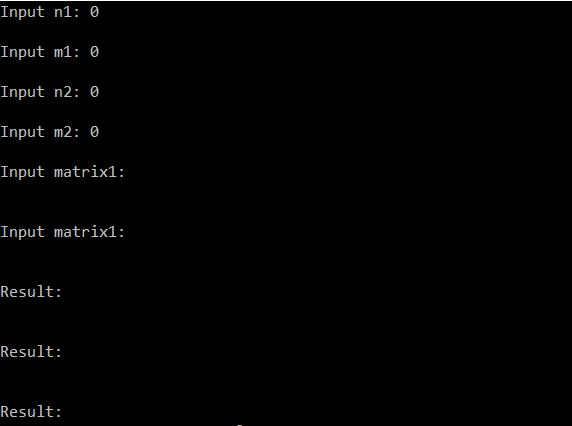
\includegraphics[width=1\linewidth]{matrix00.jpg}
\caption{Пример работы алгоритма с матрицами размерностью 0 на 0}
\label{fig:mpr}
\end{figure}

\begin{figure}[h]
\centering
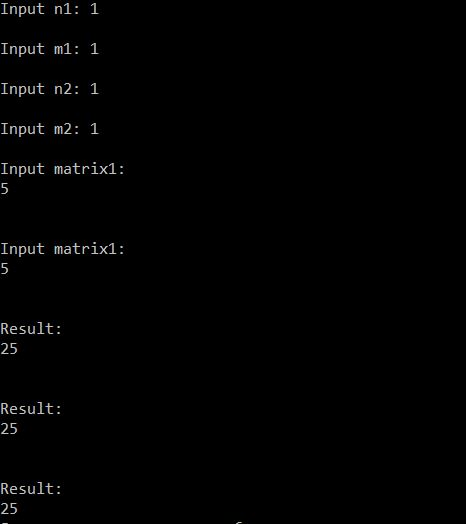
\includegraphics[width=1\linewidth]{matrix11.jpg}
\caption{Пример работы алгоритма с матрицами размерностью 1 на 1}
\label{fig:mpr}
\end{figure}

\begin{figure}[h]
\centering
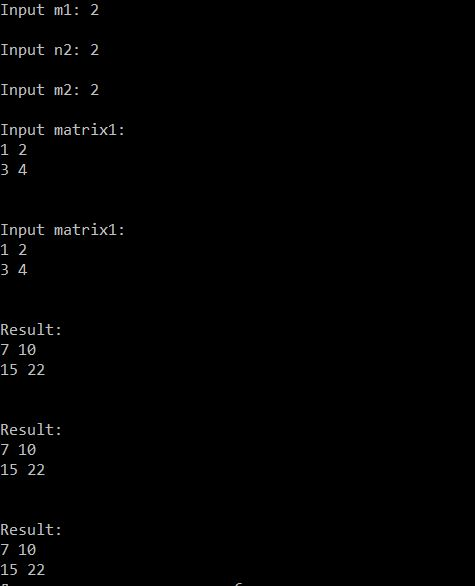
\includegraphics[width=1\linewidth]{matrix22.jpg}
\caption{Пример работы алгоритма с матрицами размерностью 2 на 2}
\label{fig:mpr}
\end{figure}

\begin{figure}[h]
\centering
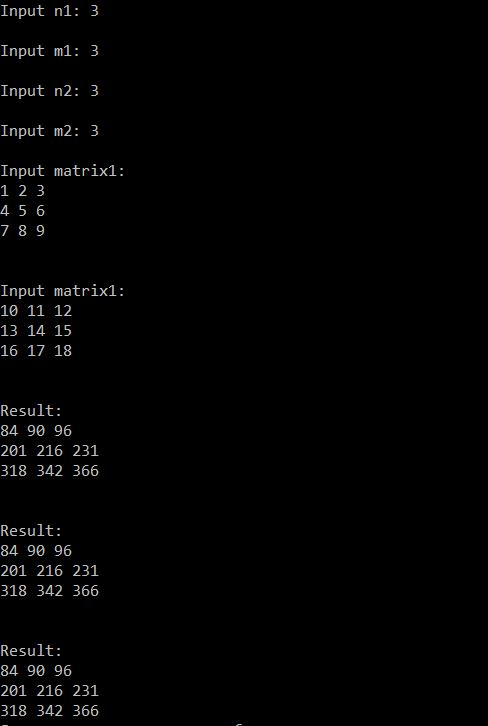
\includegraphics[width=1\linewidth]{matrix33.jpg}
\caption{Пример работы алгоритма с матрицами размерностью 3 на 3}
\label{fig:mpr}
\end{figure}





\chapter*{Заключение}
\addcontentsline{toc}{chapter}{Заключение}
В ходе лабораторной работы я изучила алгоритмы умножения матриц: стандартный и алгоритм Винограда, оптимизировала алгоритм Винограда, дала теоретическую оценку базового алгоритма умножения матриц, алгоритма Винограда и улучшенного алгоритма Винограда, реализовала три алгоритма умножения матриц на языке программирования и сравнила алгоритмы умножения матриц.




\end{document}